\section{Firma Digitale}

La firma digitale è una tecnologia con cui possono essere
effettivamente soddisfatti tutti i requisiti richiesti per dare validità
legale ad un documento elettronico firmato digitalmente;
garantisce i servizi di integrità, autenticazione e non ripudio.
Firmare non è esattamente codificare: firmare digitalmente un documento è spesso
utile perché evita di
codificare l'intero file in quanto ciò può richiedere un
tempo elevato. Verificare una firma, quindi, non significa
decodificare.

\begin{figure}[H]
    \centering
    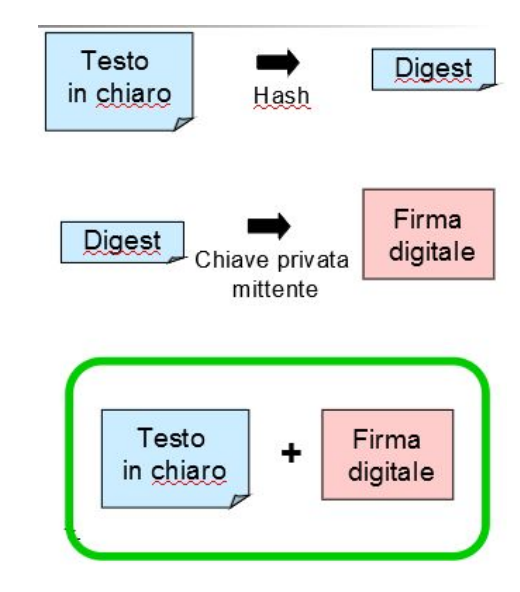
\includegraphics[width=8cm, keepaspectratio]{capitoli/crittografia/imgs/firmad.png}
\end{figure}

\subsection{Creazione della Firma}

La firma digitale viene realizzata tramite tecniche
crittografiche a
chiave pubblica insieme all'utilizzo di particolari
funzioni matematiche, chiamate funzioni hash
unidirezionali. Il processo di firma digitale passa
attraverso tre fasi:

\begin{enumerate}
    \item Generazione dell'impronta digitale.
    \item Generazione della firma.
    \item Apposizione della firma.
\end{enumerate}

Nella prima fase viene applicata al documento in
chiaro una funzione di hash appositamente
studiata che produce una stringa binaria di
lunghezza costante e piccola, normalmente 128 o 160
bit, chiamata “digest message”, ossia impronta
digitale.
Poiché la dimensione del digest message è fissa,
e molto più piccola di quella del messaggio
originale, la generazione della firma risulta
estremamente rapida. Utilizzare le funzioni hash
consente di evitare che per la generazione della
firma sia necessario applicare l'algoritmo di
cifratura all'intero testo che può essere molto lungo.
Mediante un software adatto si genera una coppia di
chiavi da utilizzare: una che verrà mantenuta
segreta per l'apposizione della firma; l'altra, destinata alla verifica, che
verrà resa pubblica. Quindi
la seconda fase, la generazione della firma, consiste semplicemente nella
cifratura con la propria
chiave privata dell'impronta digitale generata in precedenza.
Nell'ultima fase, la firma digitale generata precedentemente viene aggiunta in
una posizione
predefinita, normalmente alla fine del testo del documento.
E' da tenere presente che l'apposizione della firma digitale non garantisce la
confidenzialità del
testo, perché questo viene inviato in chiaro. Serve solo a garantirne integrità
e autenticità:

\begin{itemize}
    \item \textbf{Autenticità}: Il messaggio arriva proprio da chi dice di essere il mittente;
    \item \textbf{Integrità}: Il messaggio non ha subito modifiche o manomissioni;
\end{itemize}

\subsection{Verifica della Firma}

Il destinatario ottiene testo in chiaro con apposta la firma digitale.
Per comodità viene inviata anche la chiave pubblica del mittente. A
questo punto gli step sono:

\begin{enumerate}
    \item Separare il testo dalla firma;
    \item Decodificare la firma con la chiave pubblica del mittente;
    \item Calcolare il digest del testo tramite la funzione di hash;
    \item Verificare che i due digest coincidano. In caso positivo si ha
          la conferma del fatto che il documento è integro e non è stato
          sottoposto a modifiche.
\end{enumerate}